\RequirePackage{plautopatch}
\documentclass[fontsize = 12pt]{jlreq}
%%%%%%
\usepackage{graphicx, float}
\usepackage[font=small]{caption}
\usepackage{amsmath}
\usepackage{listings}
\usepackage{xcolor}
\definecolor{codegray}{gray}{0.6}
\lstset{%
frame=single,
rulecolor=\color{codegray},
basicstyle=\small\ttfamily,
tabsize=4,
breaklines=true, 
postbreak=\mbox{\textcolor{teal}{$\hookrightarrow$}\space}, 
float=[H], 
}

%%%%%%
\begin{document}
\begin{flushright}
2023年夏休みの自由研究\\
TAIYO\\

\end{flushright}
\noindent
{\Large%
\textbf{%
プログラミング(ガチ)初心者がIsingモデルのマルコフ連鎖モンテカルロシミュレーションに挑戦した話
}}

\begin{quotation}
\mbox{}\\
\indent
なんだかんだで後回しにしていたMCMC法の実践の記録を(わざわざ)残しておく。
ネットとかプログラミングの本とかにたくさんコードの例はあるけれど、物理的な部分の説明は省略されていることがほとんどなので、ここではそういうことも記す。
だから後々読み返したときに役立つだろうと思う、たぶん。
プログラミング力がついてからもう一度実践、またはコードの改善や別のプログラミング言語で再現する際の出発点にもなる。
使用言語はR(Rでやっている文献や記事が少なかった、というのもこれを書く動機にはなっている)。
\end{quotation}

\section{系の設定と戦略}

\subsection{統計力学からの復習}

正方格子系のハミルトニアンは
\begin{align} \label{eq:1.1}
E = -J \sum_{ \langle i, j \rangle } S_i S_j - H \sum_{i} S_i
\end{align}
とする。
ここに、$i$は格子点のうちの1点、$j$は$i$と隣り合う4つの点としている。
また、$S_i ,~S_j $はそれぞれ点$i,~j$でのスピン変数($S_i = \pm 1,~S_j = \pm 1$)で、$J$は交換相互作用定数、$H$は外部磁場に磁気モーメント$\mu _0$をかけて次元をエネルギーに変更したものである。

ここで、ある点Oに着目し、この点のスピン変数を$S_0 $と書く。
$H = 0$とすれば、注目した点Oについての(1)は
\begin{align} \label{eq:1.2}
E = -J S_0 (S_1 + S_2 + S_3 + S_4 )
\end{align}
と書き換えられる。
$S_1 ,\, S_2 ,\, S_3 ,\, S_4 $は格子点Oと隣り合う4つの点のスピン変数である。
言うまでもなく、$S_0 $が$1$をとればハミルトニアン(\ref{eq:1.2})は$E_\uparrow = -J (S_1 + S_2 + S_3 + S_4 )$となり、$S_0 $が$-1$をとれば$E_\downarrow = J (S_1 + S_2 + S_3 + S_4 )$となる。

点OのIsingスピン$S_0$が上向きをとる確率$P_\uparrow $は、カノニカル分布における確率の計算により、
\begin{align}
P_\uparrow &= \frac{\exp[-\beta E_\uparrow]}{\exp[-\beta E_\uparrow] + \exp[- \beta E_\downarrow] } \notag \\
&= \frac{1}{1 + \exp[-\beta (E_\downarrow - E_\uparrow)]} \notag \\
&= \frac{1}{1 + \exp[-2 \beta J (S_1 + S_2 + S_3 + S_4)]} \notag \\
&= \frac{1}{1 + C^{-(S_1 + S_2 + S_3 + S_4 )}} \label{eq:1.3}
\end{align}
となる。
秩序変数$C := e^{2 \beta J} = e^{2J/{kT}}$を定義した($k$はボルツマン定数、$T$は絶対温度)。

\subsection{戦略} \label{s:1.2}

ここまでの設定をRでのシミュレーションに持ち込む。
今回おこなったのは一応「シングルスピンフリップ法」という名のついた手法らしいのだが、だいぶ自己流で野蛮なものになった。

概略はこうだ。
(a)~$N \times N$の正方格子を用意し、各点にははじめ、ランダムにスピン変数$1$と$-1$をふっておく。
(b)~次に、($S_0$にあたる)1点を無作為に選択し、その周囲4つのスピン変数からスピンが上を向く確率$P_\uparrow$を(3)で計算する。
そして選んだ点を確率$P_\uparrow$で上向きに、確率$P_\downarrow = 1 - P_\uparrow$で下向きに変更(もともとその方向を向いていたなら放置)する。
(b)を繰り返す。

\section{ソースコードとその説明}

\subsection{全体}

はじめに、このシミュレーションで使用したソースコードを(コピペの民のために)まとめて提示する。
\begin{lstlisting}
    #2nd September 2023
    #first trial making Ising model simulation
    
    library(ggplot2)
    library(gganimate)
    
    #clear screen
    rm(list = ls())
    
    #格子の長さ(要設定)
    N = 500
    A = N*N
    
    #constant
    H = 0 #magnetic field
    J = 10^{-21} #exchange interaction constant
    T = 50 #absolute temperature(K)
    k = 1.380649 * 10^{-23} #Boltzmann  constant
    
    #order parameter C
    #C = exp(2 * J / (k * T))
    C = 100 + sqrt(2)
    
    #the number of frames
    t = 1000000
    
    #initial state (random numbers)
    spin = matrix(sample(size = A, x = c(-1,1), replace = T), N, N)
    #spin = matrix(sample(size = A, x = c(-1,1), replace = T), N, N)
    
    #covert to data frame
    df_spin = data.frame(
      i_y = rep(1:N, times = N), 
      i_x = rep(1:N, each = N), 
      spin = as.vector(spin), 
      label = as.factor(paste0("iter:", 0, ", rate:", sum(spin) / N^2))
    )
    
    #heat map at initial state
    ggplot(df_spin, aes(x = i_x, y = i_y, fill = spin)) +
      geom_tile() +
      xlab("") +
      ylab("") +
      scale_fill_gradient(low = "white", high = "black") +
      theme_bw() +
      coord_fixed(ratio = 1) +
      theme(legend.position = "none")
    
    #chose a point 0 in a random manner
    random_x = as.integer(runif(t, min = 1, max = N + 1)) #x coordinate
    random_y = as.integer(runif(t, min = 1, max = N + 1)) #y coordinate
    random_prob = runif(t) #random number between zero and one
    
    #probability (up)
    prob_up = function(sum_spin){
      y = 1 / (1 + C^sum_spin )
      return(y)
    }
    
    #simulate
    for(i in 1:t){
      #boundary condition
      if(random_x[i] == 1){
        random_x_exc1 = N + 1
      }else{
        random_x_exc1 = random_x[i]
      }
      if(random_y[i] == 1){
        random_y_exc1 = N + 1
      }else{
        random_y_exc1 = random_y[i]
      }
      if(random_x[i] == N){
        random_x_exc2 = 0
      }else{
        random_x_exc2 = random_x[i]
      }
      if(random_y[i] == N){
        random_y_exc2 = 0
      }else{
        random_y_exc2= random_y[i]
      }
      
      #sum four spin variables around point o
      sum_S = - spin[random_x_exc1 - 1, random_y[i]] - spin[random_x_exc2 + 1, random_y[i]] - spin[random_x[i], random_y_exc1 - 1] - spin[random_x[i], random_y_exc2 + 1]
      
      #replace S_0
      if(random_prob[i] < prob_up(sum_S)){
        spin[random_x[i], random_y[i]] = 1
      }
      else{
        spin[random_x[i], random_y[i]] = -1
      }
    }
    
    #covert to data frame
    df_spin = data.frame(
      i_y = rep(1:N, times = N), 
      i_x = rep(1:N, each = N), 
      spin = as.vector(spin), 
      label = as.factor(paste0("iter:", 0, ", rate:", sum(spin) / N^2))
    )
    
    #heat map at final state
    ggplot(df_spin, aes(x = i_x, y = i_y, fill = spin)) +
      geom_tile() +
      xlab("") +
      ylab("") +
      scale_fill_gradient(low = "white", high = "black") +
      theme_bw() +
      coord_fixed(ratio = 1) +
      theme(legend.position = "none")
\end{lstlisting}

\subsection{詳細な情報}

ここからは上で示したプログラムの詳細の説明である。

使用したパッケージは次の通り:
\begin{lstlisting}
    library(tidyverse)
    library(gganimate)
\end{lstlisting}
説明不要ではあるが、
\begin{lstlisting}
    #clear screen
    rm(list = ls())
\end{lstlisting}
も重要である(ここら辺のお作法は\cite{生命}から学んだ)。

次に、実行毎に変更・調整が必要な系の設定である。
1辺あたりの格子点の数$N$と格子全体での点の数$A$を次のように決める:
\begin{lstlisting}
    #格子の長さ(要設定)
    N = 100
    A = N*N
\end{lstlisting}
定数諸々は次のとおり(適宜変更が必要):
\begin{lstlisting}
    #constant
    H = 0 #magnetic field
    J = 10^{-21} #exchange interaction constant
    T = 50 #absolute temperature(K)
    k = 1.380649 * 10^{-23} #Boltzmann  constant
\end{lstlisting}
$J$の値は物質によるのだろうが詳しい値は調べなかった(というか調べたけれど分からなかった)。
これらの値を用いて秩序定数$C$を決定する:
\begin{lstlisting}
    #order parameter C
    C = exp(2 * J / (k * T))
    #C = 3
\end{lstlisting}
3行目のように手っ取り早く値を決定してしまってもよいかもしれない。
ちなみに、厳密に$C = 1 + \sqrt{2}$が臨界点\cite{田崎統計}。

気は早いがここでシミュレーションの最大試行回数(これが、\ref{s:1.2}節の(b)で格子点をランダムサンプリングした回数)を設定しておく:
\begin{lstlisting}
    #the number of frames
    t = 1000000
\end{lstlisting}
なかなか収束してくれないし、かといってこの値を大きくしすぎると時間を食うから何が最適解なのか知りたい(未来の自分へ)。

正方格子に初期配置としてスピン変数$S$をランダムにばらまく:
\begin{lstlisting}
    #initial state (random numbers)
    spin = matrix(sample(size = A, x = c(-1,1), replace = T), N, N)
\end{lstlisting}
\texttt{sample()}は「\texttt{c(-1,1)}からデータを\texttt{A}個取ってきなさい」という命令だが、当然\texttt{c(-1,1)}には元が2つしかないので$A \ge 2$に対しては足りなくて困っちゃう(ToT)。
\texttt{replace = T}というのは、元を抜き取るたびに\texttt{c(-1,1)}の元をリセットし$1$と$-1$を用意しておく、という役割を果たしている。

ヒートマップ作成の事前準備として、先程定義した行列\texttt{spin}をデータフレームに変更する:
\begin{lstlisting}
    #covert to data frame
    df_spin = data.frame(
        i_y = rep(1:N, times = N), 
        i_x = rep(1:N, each = N), 
        spin = as.vector(spin), 
        label = as.factor(paste0("iter:", 0, ", rate:", sum(spin) / N^2))
    )
\end{lstlisting}
ggplotによるヒートマップの作成:
\begin{lstlisting}
    #heat map at initial state
    ggplot(df_spin, aes(x = i_x, y = i_y, fill = spin)) +
        geom_tile() +
        xlab("") +
        ylab("") +
        scale_fill_gradient(low = "white", high = "black") +
        theme_bw() +
        coord_fixed(ratio = 1) +
        theme(legend.position = "none")
\end{lstlisting}
結果は次のようになる。
\begin{figure}[H] 
    \centering 
    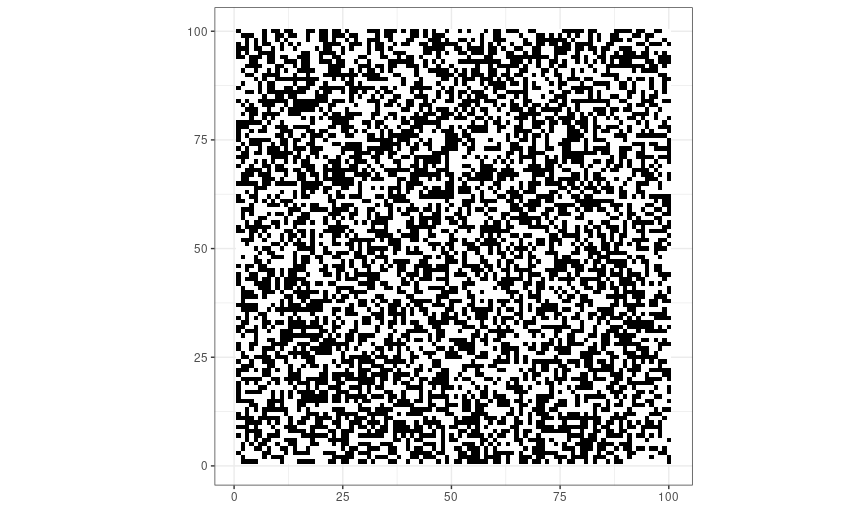
\includegraphics[width=15cm]{f1.png}
\end{figure}%

いよいよ、\ref{s:1.2}節(b)で方針を示したシミュレーションを実行する。
\texttt{spin}行列の点$(x, y)$をランダムに抽出する。
$x$座標と$y$座標それぞれについて$t$回分の乱数を生成してベクトル\texttt{random\_x}とベクトル\texttt{random\_y}に格納した:
\begin{lstlisting}
    #chose a point 0 in a random manner
    random_x = as.integer(runif(t, min = 1, max = N + 1)) #x coordinate
    random_y = as.integer(runif(t, min = 1, max = N + 1)) #y coordinate
\end{lstlisting}
点Oのスピンを反転させるかの決定に使う確率も今のうちに用意しておく。
つまり、0以上1未満の実数である元を$t$個もつベクトルを作成する:
\begin{lstlisting}
    random_prob = runif(t) #random number between zero and one
\end{lstlisting}

$S_0$が$1$をとる確率(\ref{eq:1.3})を出力する関数\texttt{prob\_up}を用意する:
\begin{lstlisting}
    #probability (up)
    prob_up = function(sum_spin){
        y = 1 / (1 + C^delta_spin )
        return(y)
    }
\end{lstlisting}
引数\texttt{sum\_spin}は(\ref{eq:1.3})に現れた$S_1 + S_2 + S_3 + S_4 $である。

$S_0$の置き換えを実行する:
\begin{lstlisting}
    #simulate
    for(i in 1:t){
        #boundary condition
        if(random_x[i] == 1){
            random_x_exc1 = N + 1
        }else{
            random_x_exc1 = random_x[i]
        }
        if(random_y[i] == 1){
            random_y_exc1 = N + 1
        }else{
            random_y_exc1 = random_y[i]
        }
        if(random_x[i] == N){
            random_x_exc2 = 0
        }else{
            random_x_exc2 = random_x[i]
        }
        if(random_y[i] == N){
            random_y_exc2 = 0
        }else{
            random_y_exc2= random_y[i]
        }

        #sum four spin variables around point o
        sum_S = - spin[random_x_exc1 - 1, random_y[i]] - spin[random_x_exc2 + 1, random_y[i]] - spin[random_x[i], random_y_exc1 - 1] - spin[random_x[i], random_y_exc2 + 1]
  
        #replace S_0
        if(random_prob[i] < prob_up(sum_S)){
            spin[random_x[i], random_y[i]] = 1
        }
        else{
            spin[random_x[i], random_y[i]] = -1
        }
    }
\end{lstlisting}
これはとても長いので、順を追って説明する。
\texttt{for}文によって$t$回の点0ランダム抽出、スピン変数置換判定をおこなう。
系の内部での変化に集中したいので、周期境界条件を課した。
すなわち、$S_{N+1} = S_1$とした(紙をトーラス形に折りたたんだ時のつなぎ目をイメージするのが分かりやすいと思う)。
4つの\texttt{if}文がそれを司る。
1つ目の\texttt{if}は、$x$座標が1の場合の対策である。
$x -1 = 1 - 1 = 0$を$N$に校正するために、$x = 0$の場合には$x = N+1$という置き換えをした。
2つ目の\texttt{if}は、$y$座標が1の場合の対策である。
$x = 1$の場合と同じ仕組みを利用した。
3つ目の\texttt{if}は、$x$座標が$N$の場合の対策である。
$x + 1 = N + 1$を1に校正するために、$x = 0N$の場合には$x = 0$という置き換えをした。
4つ目の\texttt{if}は、$y$座標が$N$の場合の対策である。
$x = N$の場合と同じ仕組みを利用した。
ここの境界条件のコードは絶対にもっとエレガントな方法があると思うので、思いついたら更新したい。

\texttt{if}文で境界条件を設定し終えたら、$S_0$の周りの4つのスピン変数の和\texttt{sum\_S}を計算する。

そして、\texttt{if}文を用いて、あらかじめ用意しておいた0以上1未満の実数\texttt{rndom\_prob[1]}が関数\texttt{prob\_up()}で計算しておいたスピンが上を向く確率より小さい時に、スピン変数$S_0$を1に変更する。
逆に\texttt{rndom\_prob[1]}が\texttt{prob\_up()}以上である場合にはスピン変数$S_0$を$-1$に変更する。
これで、点Oのスピンを確率\texttt{prob\_up()}で上向きに変更することができる。

次に、上のコードで再編集された行列\texttt{spin}をデータフレームに変換する:
\begin{lstlisting}
    #covert to data frame
    df_spin = data.frame(
        i_y = rep(1:N, times = N), 
        i_x = rep(1:N, each = N), 
        spin = as.vector(spin), 
        label = as.factor(paste0("iter:", 0, ", rate:", sum(spin) / N^2))
    )
\end{lstlisting}

作成したデータフレームからシミュレーション実行後の系の状態をヒートマップで記す:
\begin{lstlisting}
    #heat map at final state
    ggplot(df_spin, aes(x = i_x, y = i_y, fill = spin)) +
        geom_tile() +
         xlab("") +
         ylab("") +
         scale_fill_gradient(low = "white", high = "black") +
         theme_bw() +
         coord_fixed(ratio = 1) +
         theme(legend.position = "none")
\end{lstlisting}
下図が、系の最終状態の様子(の例)。
もちろんこれが収束している状態とは限らないので、必要ならば最大試行回数$t$の値を大きくしたり、コードの\texttt{\#simulate}以下の部分をもう何回か繰り返すなどが必要だ。
\begin{figure}[H] 
    \centering 
    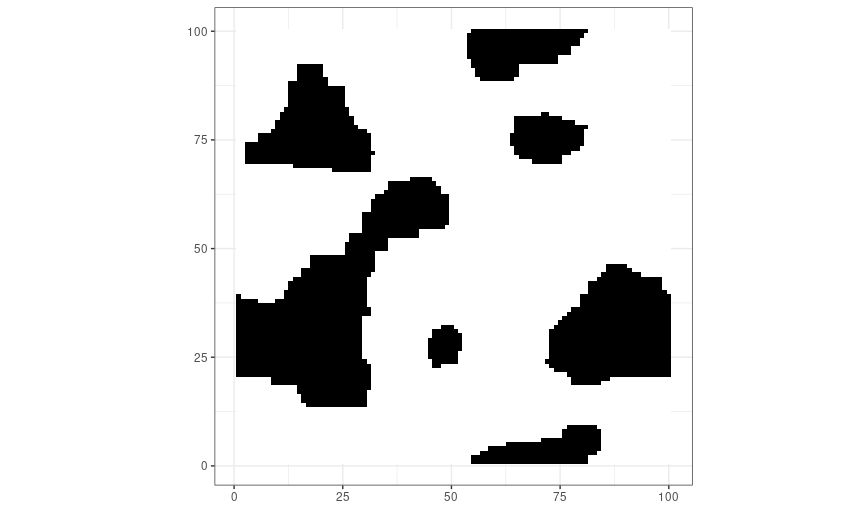
\includegraphics[width=15cm]{f2.png}
\end{figure}%

\begin{thebibliography}{99}
\bibitem{生命} 富永大介訳、Andrew P. Beckerman, Dylan Z. Childs, Owen L. Petchey:『Rをはじめよう 生命科学のためのRstudio入門』(羊土社 2019年)。
\bibitem{田崎統計} 田崎晴明:『統計力学Ⅱ』(培風館 2008年)。
\end{thebibliography}

\end{document}